\begin{figure}[!p]
    \centering
    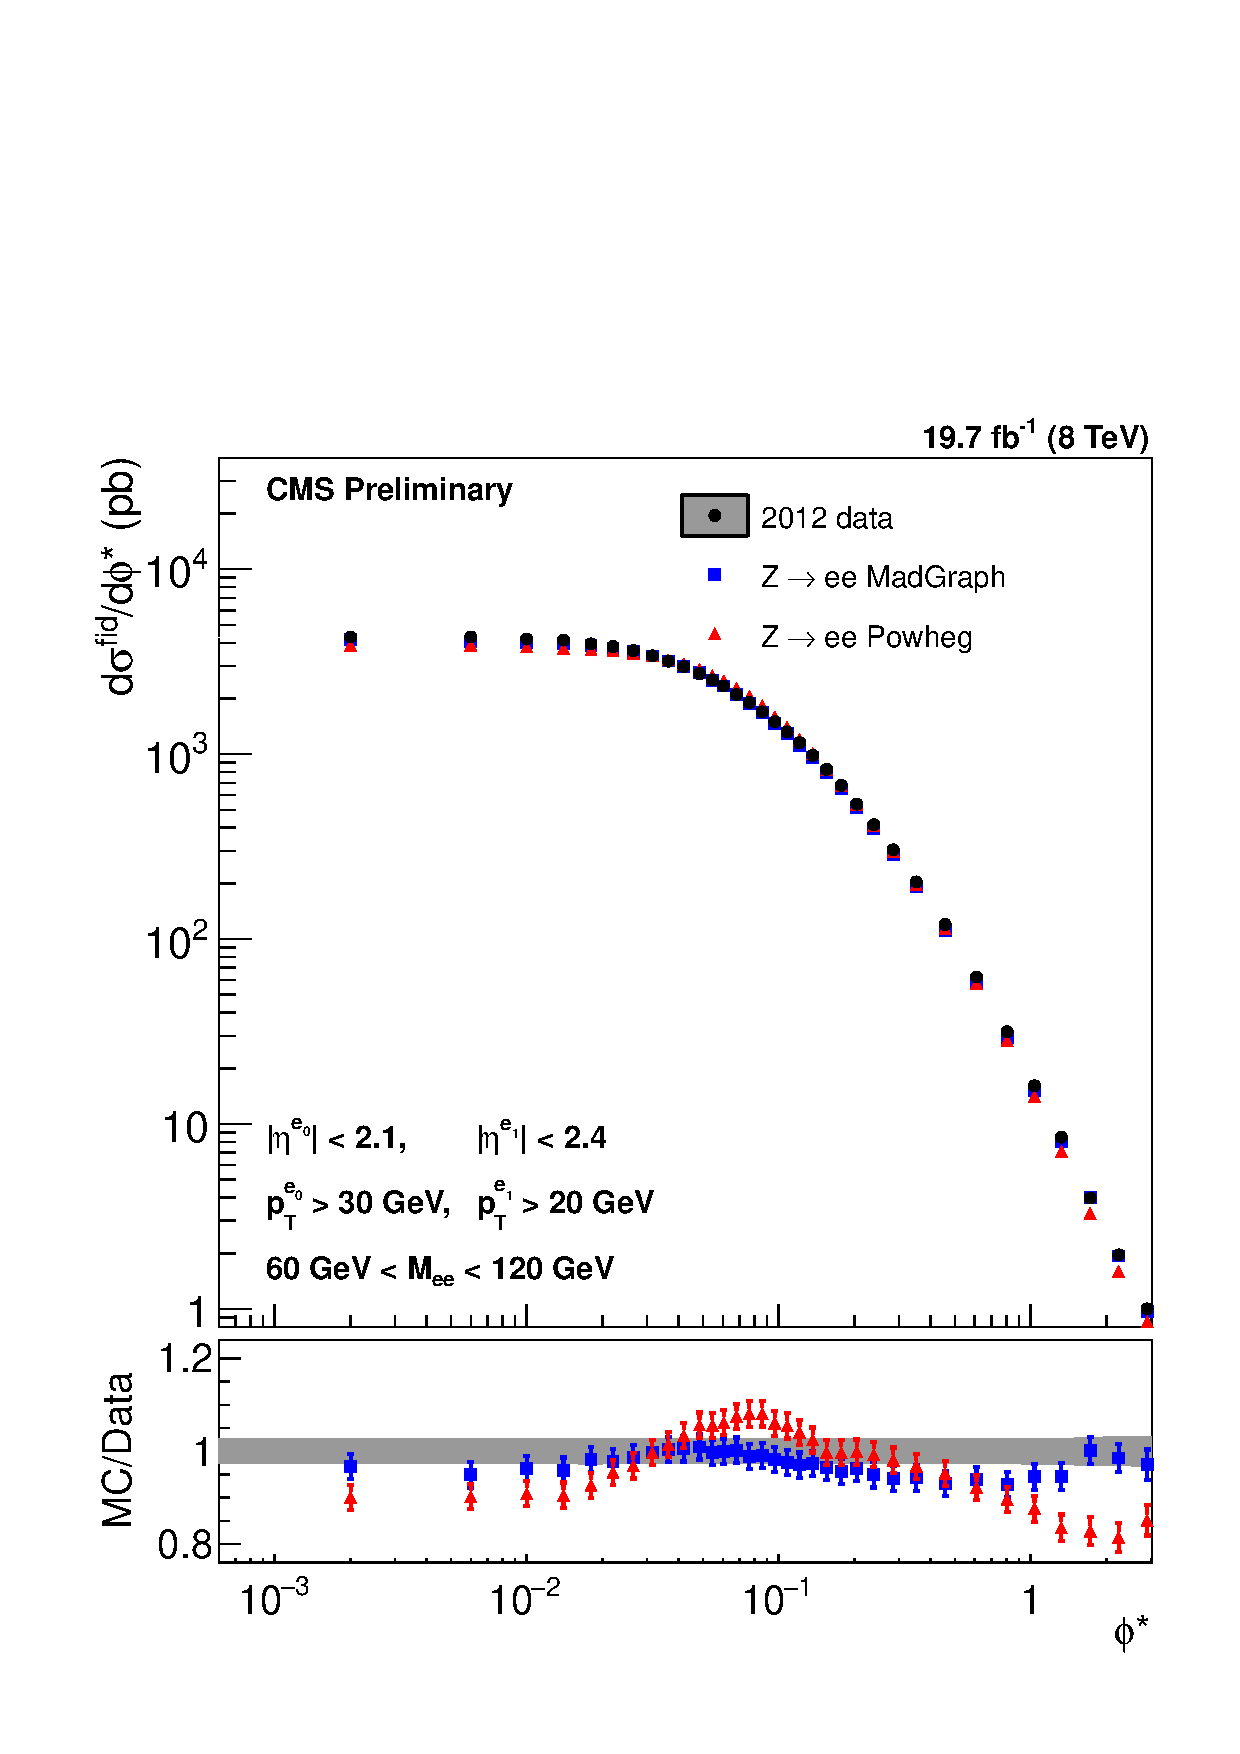
\includegraphics[width=\textwidth]{figures/ZShape_elec_Abs_Dressed.pdf}
    \caption[
        The absolute differential cross section with respects to \phistar for
        \Ztoee events in our fiducial region from data and \MADGRAPH and
        \POWHEG.
    ]{
        The absolute differential cross section with respects to \phistar for
        \Ztoee events in our fiducial region from data and \MADGRAPH and
        \POWHEG. A close up of the lower plot is shown in
        \FIG~\ref{fig:results_ratio_abs}.
    }
    \label{fig:results_abs}
\end{figure}

\begin{figure}[!p]
    \centering
    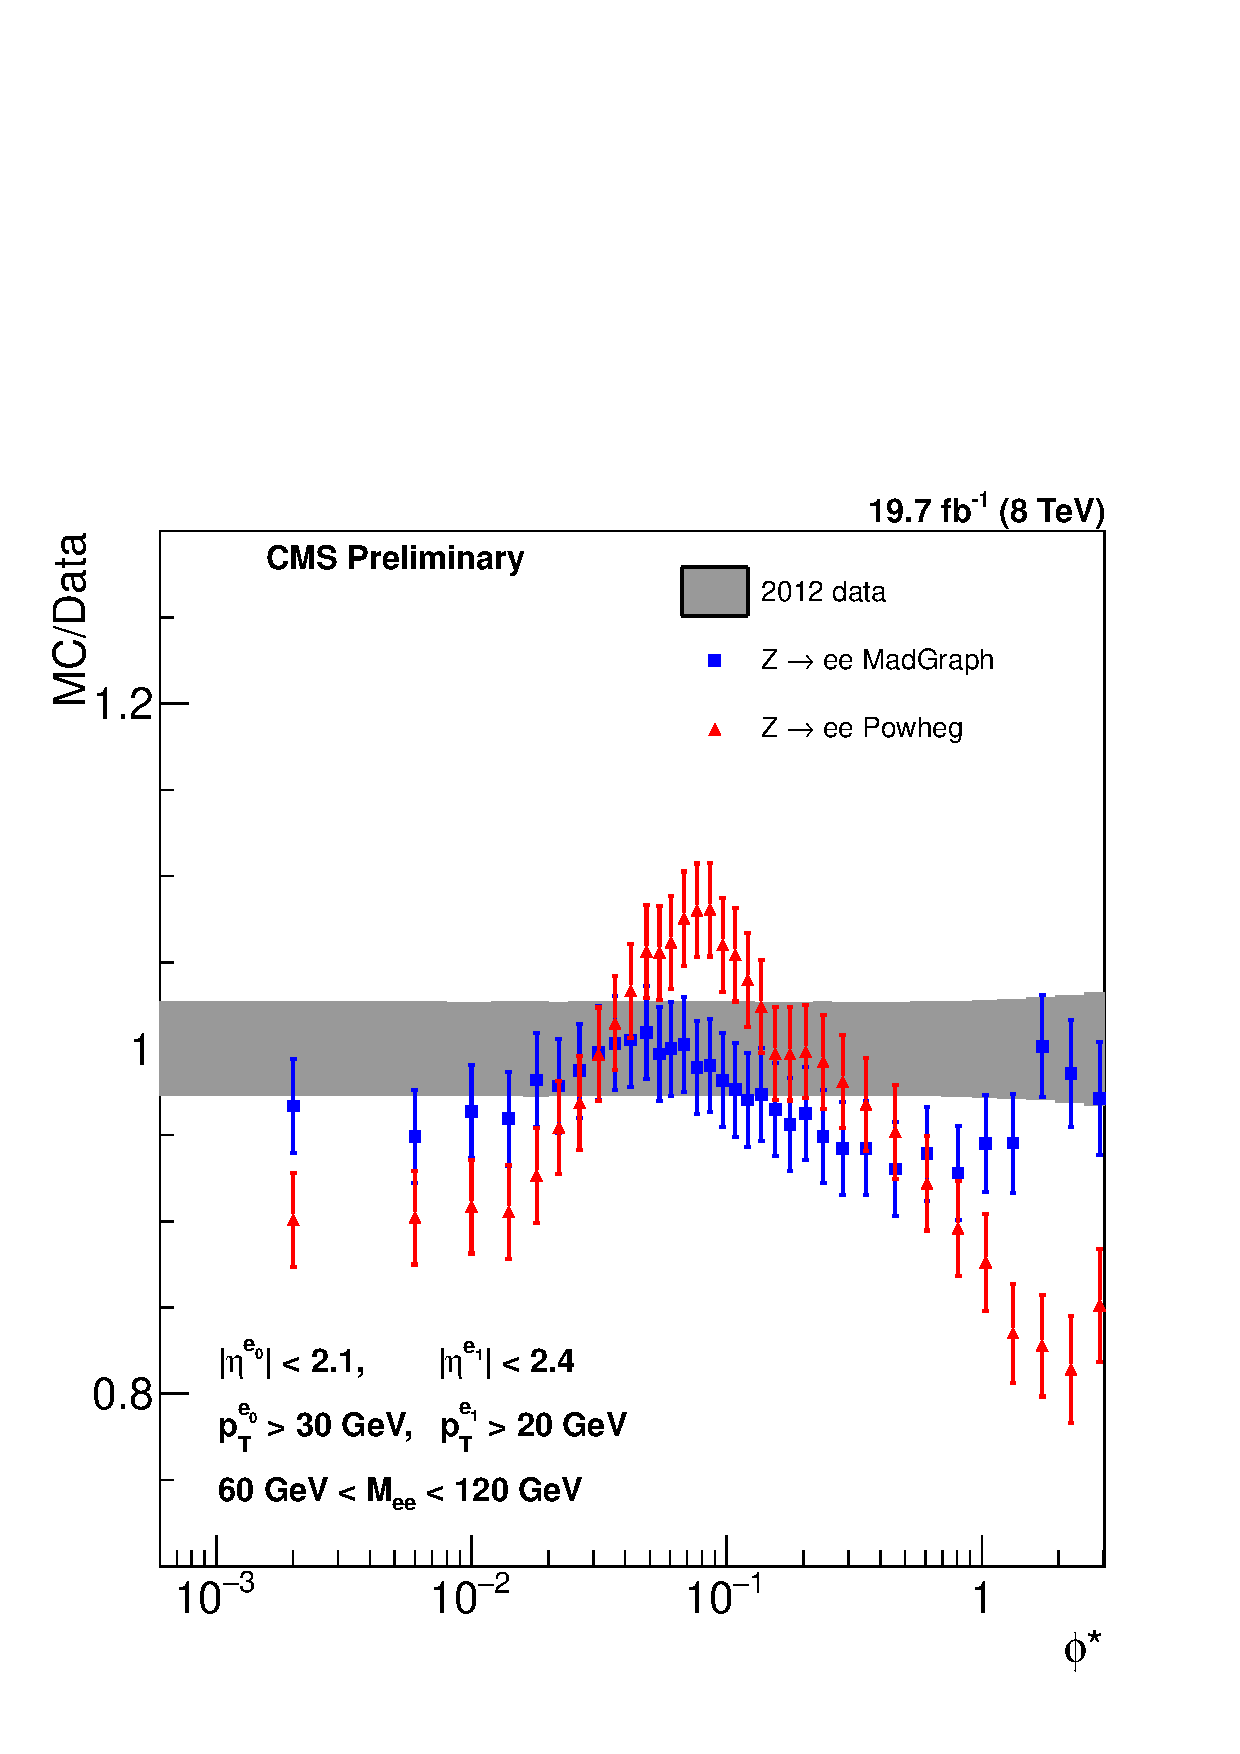
\includegraphics[width=\textwidth]{figures/ZShape_Ratioelec_Abs_Dressed.pdf}
    \caption[
        Close up of the ratio plot from \FIG~\ref{fig:results_abs} for the
        absolute cross section measurement.
    ]{
        Close up of the ratio plot from \FIG~\ref{fig:results_abs} for the
        absolute cross section measurement. The error band indicates the
        uncertainty in the data, while the square points show the ratio of
        \MADGRAPH over data, and the triangle points show the ratio of \POWHEG
        over data.
    }
    \label{fig:results_ratio_abs}
\end{figure}
